\begin{figure}[htbp]
\section*{ TGFBR1}
\centering
\begin{subfigure}[b]{0.95\textwidth}
\centering
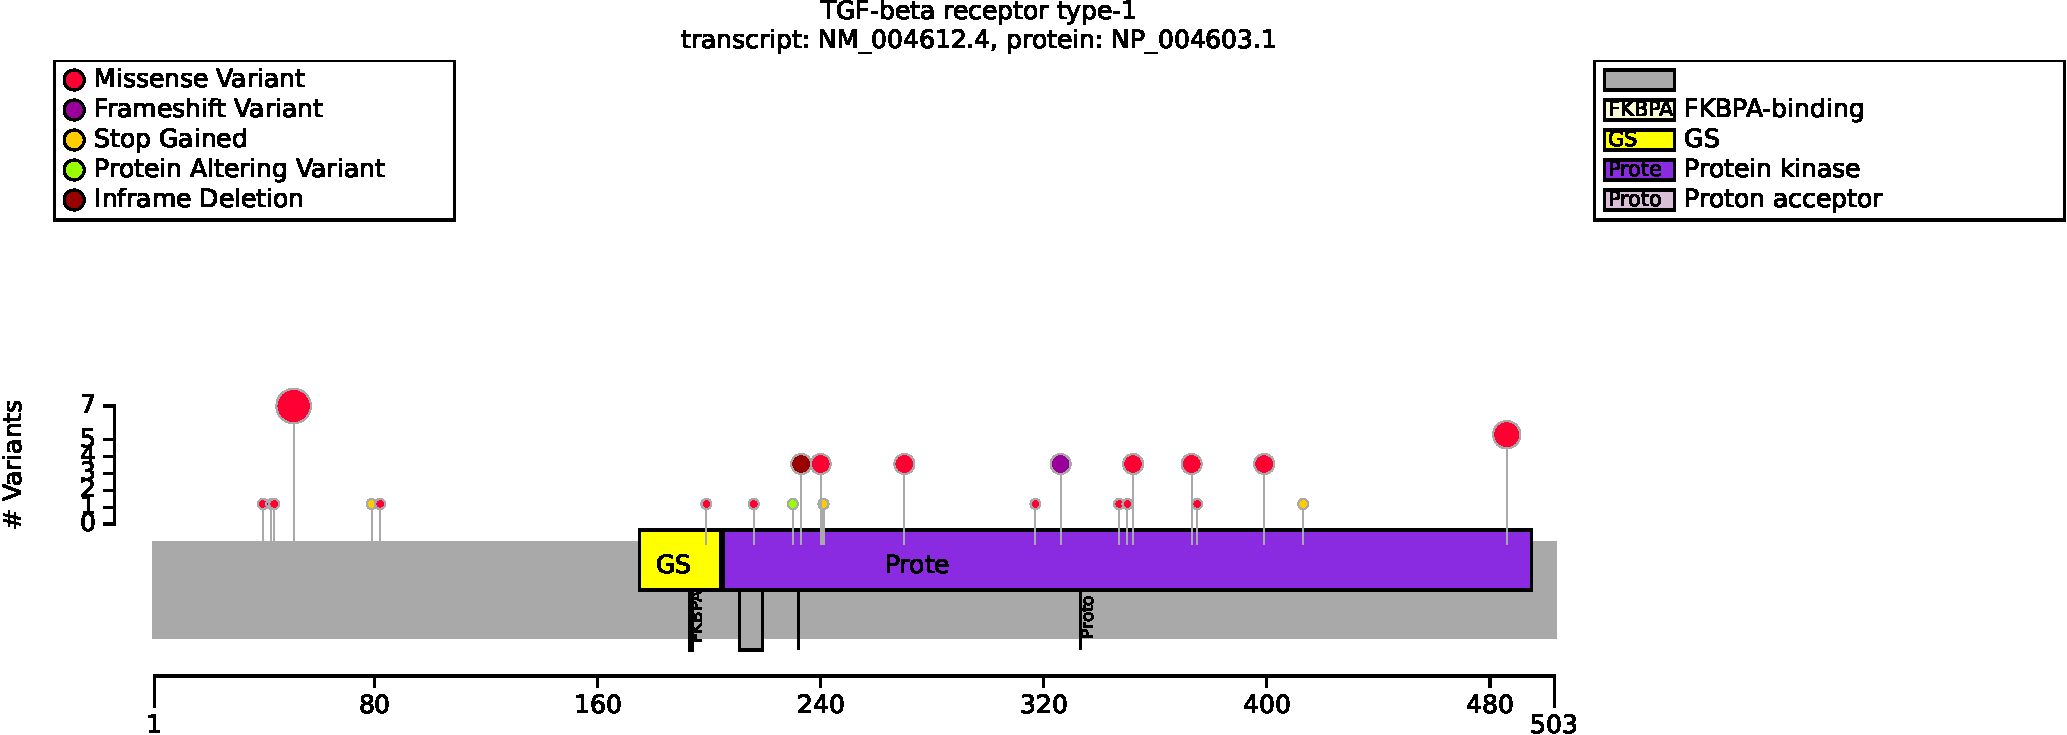
\includegraphics[width=\textwidth]{ img/TGFBR1_protein_diagram.pdf} 
\captionsetup{justification=raggedright,singlelinecheck=false}
\caption{Distribution of variants in TGFBR1}
\end{subfigure}

\vspace{2em}

\begin{subfigure}[b]{0.95\textwidth}
\centering
\resizebox{\textwidth}{!}{
\begin{tabular}{llllrr}
\toprule
HPO term & MSSE var & other & p-value & adj. p-value\\
\midrule
Self-healing squamous epithelioma [HP:0034720] & 18/19 (95\%) & 0/21 (0\%) & $1.68\times 10^{-10}$ & $2.01\times 10^{-9}$\\
Hypertelorism [HP:0000316] & 0/18 (0\%) & 15/19 (79\%) & $5.01\times 10^{-7}$ & $3.01\times 10^{-6}$\\
Arterial tortuosity [HP:0005116] & 1/19 (5\%) & 8/16 (50\%) & 0.005 & 0.020\\
\bottomrule
\end{tabular}
}
\captionsetup{justification=raggedright,singlelinecheck=false}
\caption{Fisher Exact Test performed to compare HPO annotation frequency with respect to MSSE var and other. Total of
        12 tests were performed. }
\end{subfigure}
\vspace{2em}
\begin{subfigure}[b]{0.95\textwidth}
\centering
\resizebox{\textwidth}{!}{
\begin{tabular}{llllrr}
\toprule
HPO term & Gly52Arg & Other & p-value & adj. p-value\\
\midrule
Self-healing squamous epithelioma [HP:0034720] & 7/7 (100\%) & 11/33 (33\%) & 0.002 & 0.005\\
Hypertelorism [HP:0000316] & 0/7 (0\%) & 15/30 (50\%) & 0.028 & 0.042\\
\bottomrule
\end{tabular}
}
\captionsetup{justification=raggedright,singlelinecheck=false}
\caption{Fisher Exact Test performed to compare HPO annotation frequency with respect to Gly52Arg and Other. Total of 3 tests were performed.}
\end{subfigure}
\vspace{2em}
\begin{subfigure}[b]{0.95\textwidth}
\centering
\resizebox{\textwidth}{!}{
\begin{tabular}{llllrr}
\toprule
Genotype (A) & Genotype (B) & total tests performed & significant results\\
\midrule
FEMALE & MALE & 16 & 0\\
\bottomrule
\end{tabular}
}
\captionsetup{justification=raggedright,singlelinecheck=false}
\caption{Fisher Exact Test performed to compare HPO annotation frequency with respect to genotypes. }
\end{subfigure}

\vspace{2em}

\caption{ The cohort comprised 41 individuals (7 females, 16 males, 18 with unknown sex). 2 of these individuals were reported to be deceased. 
A total of 78 HPO terms were used to annotate the cohort. Disease diagnoses: Loeys-Dietz syndrome 1 (OMIM:609192) (23 individuals), Multiple self-healing squamous epithelioma, susceptibility to (OMIM:132800) 
(18 individuals). A total of 41 unique variant alleles were found in \textit{TGFBR1} (transcript: \texttt{NM\_004612.4}, protein id: \texttt{NP\_004603.1}).
Goudie et al. (2011) reported that the nature of the sequence variants, which include mutations in the extracellular ligand-binding domain and a series of truncating mutations in the kinase domain, 
indicates a clear genotype-phenotype correlation between loss-of-function TGFBR1 mutations and MSSE \cite{PMID_21358634}.
}
\end{figure}
